\chapter{Introduction}
\label{chp:introduction}
After the introduction of the Internet on 60's and world wide web on 90's, there are more and more people connected each other using this technology. Initially, the architecture used to build the Internet is Peer-to-peer network although the most popular one is \textit{client and server}. A \textit{server} holds the content and delivers it to a user at the \textit{client} side, thus burden the server. Currently, recent research shows that peer-to-peer Internet already back at its prime by dominating the traffic\cite{2015:internettraffic:sandvine}.

Interaction among user in the Internet community can be expressed in various fashion. Peer-to-peer (P2P) is one of the major interaction existed in the net. This shown in figure \ref{fig:usage}. Many applications and protocols run on top of P2P system, online gaming, computing, and the most popular one, file sharing. \bt~is by far the most popular system used in file-sharing community with its unique \textit{tit-for-tat} mechanism to discourage uncooperative peers \cite{2003:bittorrent:cohen}. 

\begin{figure}[h]
	\centering
	\begin{subfigure}[b]{0.8\textwidth}
		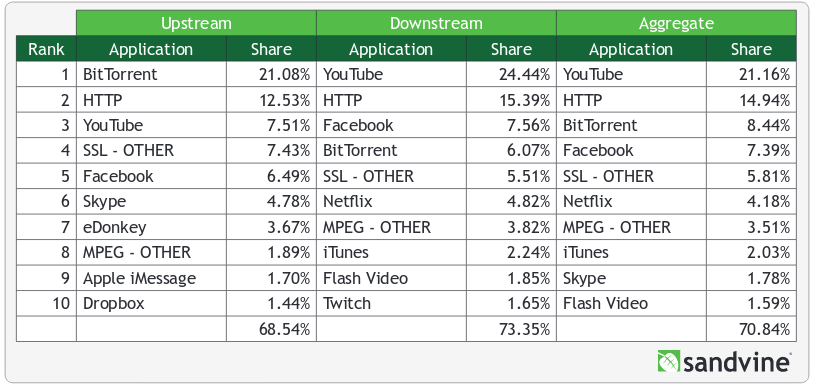
\includegraphics[width=\linewidth]{pics/sandvineeu2015}
		\caption{Sandvine data for 2015 internet usage in Europe}
		\label{fig:usage1}
	\end{subfigure}\\
	\begin{subfigure}[b]{0.8\textwidth}
		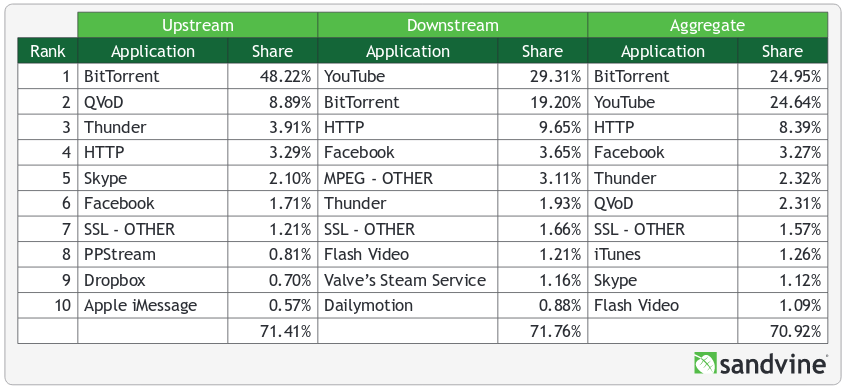
\includegraphics[width=\linewidth]{pics/sandvineasia2015}
		\caption{Sandvine data for 2015 internet usage in Asia Pasific}
		\label{fig:usage2}
	\end{subfigure}%
	\caption{Traffic of the Internet by Sandvine \cite{2015:internettraffic:sandvine}}.
	\label{fig:usage}
\end{figure}

Peer-to-peer network has many different applications. Some of them are multimedia streaming, online gaming, and file-transfer. All of those applications has different requirement to ensure the user has a flawless experience. Multimedia streaming, for example, needs to achieve two conditions. First, the start up delay must be small to make sure user do not abandon his intent to stream the files. Secondly, the chunk (or piece) loss must be negligible, or at least low enough to provide good quality\cite{2008:givetogetvod:Mol}. Other application, P2P gaming, require more complex situation. Depend on the type of the game (e.g., FPS), peer latency must be under certain threshold\cite{2010:surveyp2pgame:shen}. It also needs to consider bandwidth demand and high security to prevent cheating between user. The most common P2P application, file transfer, obviously need high throughput by maximizing all the connection a user has.

\section{The freeriding phenomenon}
Among all the peer-to-peer usage in the Internet, file-sharing is the most popular one. It started with Napster in 1999 to share music file between its users. It shut down at 2001 and immediately followed by Kazaa and Gnutella afterward. Both services allowed the user to share not only music file but also another type of files. Currently, both already shut down because of legal and performance issues. In Gnutella case, the majority of users (70\%) stopped to share their files. Moreover, about half of the communication only served by top 1\% of the community \cite{2000:freeridegnutella:adar}. Gnutella suffers from a social phenomenon called \textit{freeriding} on the majority of its users.

Freerider defined as the user behavior that selfishly consumes all the resource without giving back. This behavior can cause several problems, especially in peer-to-peer network. First and foremost, freeriding behaviour can lead to vulnerabilities in the system. With only few of the user provide the service for many, it eventually becomes more centralized than decentralized system. Another well-known problem caused by freeriders is the degradation of system performance \cite{2000:freeridegnutella:adar}. \citeauthor{2000:freeridegnutella:adar} showed that lots of P2P peers are always shown self-interest and rationality that can be categorized as freeriding. If freeriders become majority in file-sharing peer-to-peer system, as they occupy significant amount of resource, eventually bottleneck in the system will occur. As the time goes, honest peer may not feel satisfied and decided to leave the system. With important peer leave the system, it will degrade more and lost the file that used to be served by leaving peer. The system becomes unhealthy and sooner or later will be completely left by its peers.

Freeriding can lead to a systematically worse problem called ``tragedy of the commons'' \cite{1968:tragedycommon:hardin}. This problem was popularized by \citet*{1968:tragedycommon:hardin} in \citeyear{1968:tragedycommon:hardin}. This social dilemma emerges because of overuse and overexploitation in the shared resource without feedback from the user. As \citeauthor{1968:tragedycommon:hardin} stated in his paper: ``Freedom in a commons brings ruin to all'', uncontrollable participant in an environment with limited shared resource could take something out of the common to fulfill their own gain.
% how can egoist cooperate :  The Emergence of Cooperation among Egoists (Robert Axelrod). Solved by tit-for-tat -> good performance. managing supply and demand meulpowder p.7

% freerider behaviour, tit-for-tat result
In \bt, one of the protocols used in file-sharing, it is unlikely a user will \textit{extremely freeride}. We define this behavior as not upload anything while keep downloading data. Instead of extremely freeriding, it is more common to find \textit{hit and run} behavior \cite{2011:managesupplydemand:meulpolder}. Hit and run (HnR) is a situation where a user has finished downloading then immediately stop his contribution. Hit and run also often referred as one of the freeriding behavior that peer-to-peer community wanted to prevent. \citeauthor{2015:freeriderinbtcommunity:das} also studied the freerider behavior in \bt~communities. They conclude that freerider in \bt~may not degrade performance as long as the swarm has at least one dedicated and available seeders. The potential availability of seeder also become a factor that keeping the swarm alive \cite{2015:freeriderinbtcommunity:das}. 
%. One thing that need to take into consideration is that in their research, they only take four communities as dataset 

\section{BitTorrent protocol}
\bt~\cite{2003:bittorrent:cohen}, nowadays, stand as \textit{de facto} file-sharing protocol on top of peer-to-peer network. It survives until now because \bt~ is a \textit{protocol} that can be implemented by anyone, instead of service that Napster, Kazaa, and Gnutella used to have. One of the open source implementation of \bt~is \textit{libtorrent}\footnote{\url{http://libtorrent.org/}}. To build a system on top of \bt~environment, it is essential to know the complete view how \bt~work. 

% tit-for-tat, choking, unchoke, optimistic unchoke
In general view, \bt~consists of peers who participated in file-sharing and \textit{tracker}. \textit{Tracker} is responsible for monitors the distribution and progress of the file and peers in the swarm. \textit{Swarm} is a set of peers formed with the same purpose of downloading or uploading certain files represented in \texttt{.torrent} metadata file. Static \texttt{.torrent} file, which contains information such as tracker addresses and unique hash value of this swarm, is created by peer who wants to publish their files. Peer uses information in \texttt{.torrent} file to connect each other. Files in a swarm consist of several \textit{chunks} or file pieces. A chunk is exchanged by the peers in a particular period. A peer actively participated in many swarms on the uninterrupted time-frame called \textit{session}.

In \bt, it is desirable to have many peers upload pieces of file to the swarm. This way, swarm can be \textit{healthier}, and overall download speed can increase. However, many peers become a \textit{leecher}, which quit the swarm when his download finished. This behavior also called as \textit{Hit and Run} (HnR) \cite{2014:sustainabilitytorrent:chen}. In general, that unwanted behavior normally forbidden in private communities. In such a community, the administrator enforces several policies such as \textit{Share Ratio Enforcement} (SRE). SRE define the amount a user need to upload before able to download from the community \cite{2012:economicbt:kash}. 

% how bittorrent handle freeriding (short term)
\bt~uses \textit{tit-for-tat} mechanism to reward good behavior and punish bad behavior. This mechanism tried to solve fairness issue introduced by freeriding behavior \cite{2003:bittorrent:cohen}. \textit{Tit-for-tat} in \bt~ encourage user to only upload file to one who also has uploaded his file somewhere else. Furthermore, it is also ranked by upload amount and speed. Freeriders always get low priority in this mechanism. In this way, \textit{tit-for-tat} incentivizes for user to upload a file. \bt~protocol and its \textit{tit-for-tat} become a standard in file-sharing peer-to-peer system with many clients implemented this protocol. \textit{Tit-for-tat} valid only in a scope of single torrent. That means, the configuration from one community can not be carried to another community. This causes \textit{tit-for-tat} works best only in short term transaction and limited parties. Nevertheless, \citeauthor{2005:bittorrentcooperation:andrade} showed that \bt~is indeed increased cooperation with only less than 10\% peer is uploading something.

\textit{Tit-for-tat} is a distinguished feature to force cooperation of other peers. By peers reciprocation, \bt~ implement \textit{choking algorithm} under this feature. It prioritizes peer who provided high upload rates. Choking algorithm is an algorithm to temporarily refuse uploading piece of file to a particular peer. Usually, an uploader has a limited number of unchoked slots. By observing other peers, choking algorithm decides which peer a particular piece will be sent or not sent to. If we unchoke a peer, it means we consider to upload a piece to that peer. For starters, it is usually useful to execute \textit{optimistic unchoking} \cite{2003:bittorrent:cohen}. Optimistic unchoking is an algorithm to unchoke a peer regardless of its activity in a swarm. This gives a peer a chance to increase his upload rate by providing more content. As for downloading, a peer picks \textit{rarest-first} chunk based on the availability in the swarm. This technique makes sure that a complete file is distributed in the swarm.

There are a lot of \bt~\textit{communities} that served as a portal to stored \texttt{.torrent} file. A community usually has their own tracker. In general, community in \bt~ can be divided into two categories: \textit{public} and \textit{private}. Public tracker means everybody can join the swarm served by that tracker. In the other hand, private communities are closed community which can be accessed by passing particular requirement \cite{2010:pubpriv:meulpolder, 2014:sustainabilitytorrent:chen}. Typically, public communities have lower performance compared to private communities \cite{2010:pubpriv:meulpolder}. \textit{Private community} typically has higher seeder-to-leecher ratio (SLR) that determines the faster download speed \cite{2005:bittorrentcooperation:andrade}. Higher performance comes with a drawback: in private communities, it is also very difficult to get a new membership and very easy to be kicked out \cite{2013:survivepriv:jia}.

% public vs private community. compare performance
% issue in both community. Imbalance.
\citeauthor{2010:pubpriv:meulpolder} measured that private communities have 3-5 times higher download speed compared to public communities \cite{2010:pubpriv:meulpolder}. This benefit makes joining private community is typically harder compared to public community. Despite has different performance, both public and private community suffer from a similar issue: ``Poor downloading experience''. It is widely known that public community generally has low SLR which directly affect the swarm performance. In the other hand, private tracker suffers from ``\textit{poor downloading motivation}'' as described by \citeauthor{2014:sustainabilitytorrent:chen}\cite{2014:sustainabilitytorrent:chen} although private community intended to solve low SLR issue. 

%\todo{expand_:Delivery procedure} -> 

\subsection{Tribler}
\label{section:tribler}
Tribler\footnote{\url{https://www.tribler.org/}} is peer-to-peer file sharing application developed at Delft University of Technology that compatible with \bt~protocol \cite{2008:tribler:pouwelse}. Tribler focused on security, fully decentralized system, and anonymity. Starts with ABC (Another \bt~Client), Tribler currently provides content discovery, channels concept, and reputation management in fully distributed manner. With Tribler downloaded from the official repository on the latest stable release (6.5.2) reaching  78440\footnote{\url{http://www.somsubhra.com/github-release-stats/ ?username=tribler&repository=tribler} (Accessed 3 September 2016)} times, it is desired to observe the usage of CMS with an adequate user base. We believe our work will be able to increase the overall swarm throughput by donating unused bandwidth on peer upstream.

All of the Tribler main components such as end-to-end encryption, channel discovery, and many others relied in database and dissemination system called \texttt{Dispersy} \cite{2013:dispersy:zeilemaker}. Dispersy maintain and perform the communication between Tribler peers in fully decentralized manner. Dispersy able to circulate the message in one-to-one or one-to-many within a group of node called \texttt{community}. User can adapt and implement its desired \textit{community} by itself. It is including how, what, and where the communication will occur.

\begin{table}[tbp]
	\centering
	\caption{Overview of implemented Dispersy community in Tribler \cite{2016:tribler-techdebt:vos}.}
	\label{tbl:community}
	\begin{tabular}{|c|p{11cm}|}
		\hline
		\rowcolor[HTML]{EFEFEF} 
		\multicolumn{1}{|c|}{\cellcolor[HTML]{EFEFEF}{\color[HTML]{333333} \textbf{Community Name}}} & \multicolumn{1}{c|}{\cellcolor[HTML]{EFEFEF}{\color[HTML]{333333} \textbf{Purpose}}}                                                                                                                                     \\ \hline
		\textit{AllChannel}                                                                          & Used to discover new channels and to perform remote channel search operations.                                                                                                                                           \\ \hline
		\textit{BarterCast4}                                                                         & While currently disabled, this community was used to spread statistics about the upload and download rates of peers inside the network and has originally been created as a mechanism to prevent free-riding in Tribler. \\ \hline
		\textit{Channel}                                                                             & This community represents a single channel and is responsible for managing torrents and playlists inside that channel.                                                                                                   \\ \hline
		\textit{Multichain}                                                                          & This community utilizes the blockchain technology and can be regarded as the accounting mechanism that keeps track of shared and used bandwidth.                                                                         \\ \hline
		\textit{Search}                                                                              & This community contains functionalities to perform remote keyword searches for torrents and torrent collecting operations.                                                                                               \\ \hline
		\textit{(Hidden)Tunnel}                                                                      & This community contains the implementation of the Tor-like protocol that enables anonymity when downloading content and contains the foundations of the hidden seeder services protocol, used for anonymous seeding.     \\ \hline
	\end{tabular}
\end{table}

Tribler implements several Dispersy \textit{communities} on its core function. \citeauthor{2016:tribler-techdebt:vos} summarize the recent community in Tribler. Important features such as channel discovery, search within community, end-to-end Tor-like operations, and currency mechanism shown in table \ref{tbl:community}. \textit{Channel} is a collection of torrent that has extra capabilities such as vote system, spam prevention, and comment (social) attributes. Every user can create his own channel, add and remove torrent to it, and maintain its activity. Worth to mention that Tribler implemented its own reputation system to incentivize user. Reputable user will get boost from other Tribler user, so it is beneficial in its own way.

In Tribler, there were several attemps to tackle freerider issue. Give-to-Get \cite{2008:givetogetvod:Mol} is one approach in peer-to-peer streaming video system. It works by give freerider only idle bandwidth slots and therefore their download speed will much slower\footnote{\url{https://www.tribler.org/Give-To-Get/}(Accessed 22 September 2016)}. There was also reputation management implemented in \textit{BarterCast4 community}, specifically to prevent freeriding in Tribler \cite{2009:bartercast:meulpolder}. It was used to spread the statistics about upload and download rate of a particular user \cite{2016:tribler-techdebt:vos}. And lastly, there is Multichain \cite{2015:multichain:norberhuis}, the anonymous tamper-proof interaction history that works on onion routing in Tribler network.

\section{Rewarding user contribution}
\label{sec:userreward}
Freeriding behavior can be prevented by proper incentive mechanism. By showing goodness, specifically, by uploading data to others, user should get a reward. However, users are typically selfish and always tries to maximize their own benefit \cite{2015:incentivep2pgame:kang}. With unclear and non-obvious incentive mechanism, some peers who download a lot may or may not know that freeriding behavior is causing trouble for the system. Therefore, they could suffer from punishment. Reward and punishment can be in many forms such as right to download specific content, get higher or lower download speed, and social acknowledgement.

To gain the reward is not as trivial as it sounds. Reward comes with good behavior which can be done by uploading content. This requires another user to actually download the content. In a community where the punishment is significantly severe, users typically very selective of its download activity. By downloading more, a user can be suspected with bad behavior that lead to punishment. Similar situation applies if the reward is insufficient. The user who want to get reward may need to standby for a long time waiting someone to download their files \cite{2013:survivepriv:jia}. This approach is inefficient, bandwidth wasting, but commonly practicable\cite{2013:survivepriv:jia}.

Incentive mechanism is essential as it is one of the property to increase general performance. \citeauthor{2011:managesupplydemand:meulpolder} discussed several kinds of incentive mechanism techniques. The technique can be combined and complement each other. Those are : (i) direct reciprocity, (ii) indirect reciprocity, (iii) centralized reputation, (iv) decentralized reputation, and (v) currency \cite{2011:managesupplydemand:meulpolder}. \textit{Reciprocity} focused on the relationship between peers.  \textit{Reputation} technique is more straightforward. The information of user behavior in the past is stored (centralized or decentralized). This information iteratively updated and spread through all the peers. Last technique is \textit{currency} which uses \textit{credit} to incentivize user.

\bt's \textit{tit-for-tat} implements reciprocation to enforce user contribution. It is based on \textit{direct reciprocation}. However, this technique has many limitations. It used short sliding window of the recent past. Although direct reciprocation is effective for relatively short period, \citeauthor{2011:managesupplydemand:meulpolder} stated that it is unlikely that two user will encounter each other again in the near future \cite{2011:managesupplydemand:meulpolder}. Especially in a swarm with many members. This limitation can be solved by \textit{indirect reciprocity}. Other user may contribute each other based on \textit{trust system} that naturally occurred in the swarm. \citeauthor{2005:indirectreciprocity:nowak} categorized indirect reciprocity into two which shown in Figure \ref{fig:reciprocation} : upstream and downstream \cite{2005:indirectreciprocity:nowak}. In \textit{downstream} reciprocity, if one peer is observed helping another peer, the observer may have more motivation to seed. This effect is based on trust. It is natural to help the helper in a society. In \textit{uptream} reciprocity, the peer that received help will have higher chance to seed another peer. This phenomenon can be interpreted as the peer who receives the data is ``giving back'' to the community.
\begin{figure}[ht]
	\centering
	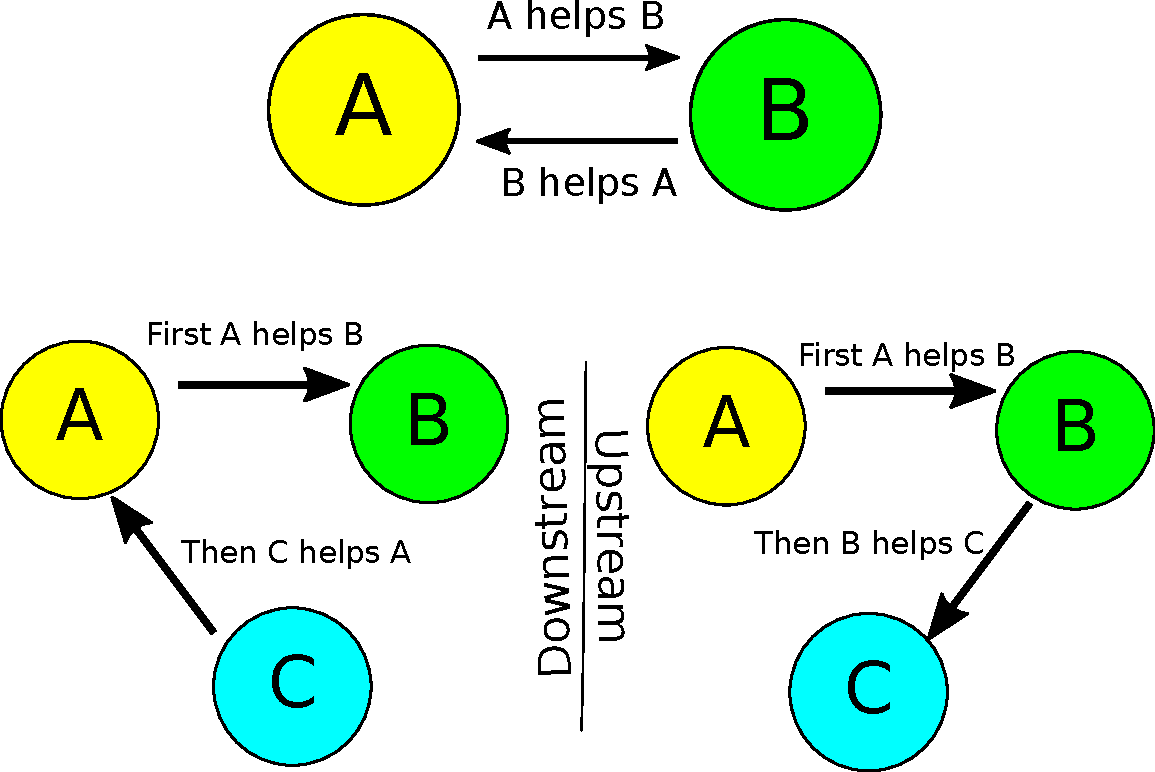
\includegraphics[width=0.7\textwidth]{pics/reciprocation.pdf}
	\caption{Direct and indirect reciprocation}
	\label{fig:reciprocation}
\end{figure}
% The focus on this thesis is to introduce credit mining system, a system to automatically upload prospected files. This system tries to find a collection of files which give relatively high reward if it uploaded in the future. As the system is implemented to increase user experience, it is implemented in such a way that it will not disturb any kind of user activities. Balancing between gaining high reward, consumed resource, and freeriding prevention become a key question of this thesis work.

\section{Economics in file-sharing}
The concept of reward and punishment can be related with the incentive mechanism used in P2P system to maintain the overall performance and to tackle the famous \textit{freeriding problem}. It is common to form the reward to user in the \textit{credit system}. Most of the private communities in \bt~employ SRE to keep the performance high. Maintain performance in P2P system is relevant with supply and demand condition in \bt~system and its misalignment problem. Credit distribution is also important as its misalignment can lead to system seize-up.

The reason why user want to have a lot of credit is motivated by advantages such as higher performance. Individual and community performance must be balanced with each other. \citeauthor{2013:survivepriv:jia} mentioned that oversupply swarm will limit the possibility of giving higher bandwidth allocation for users \cite{2013:survivepriv:jia}. This phenomenon shows that although the intention from user is good, it is not the best case for the swarm perspective. Therefore, it is important for user to choose which community he want to seed to balance those interest.

This section presents the prior knowledge needed to observe social-economic phenomenon and to apply suitable policy improving overall experience or performance. Two aspects will be elaborated : credit in currency as to incentive user, and supply and demand in the P2P community specifically \bt.

\subsection{P2P currency and incentive}
% incentive p2p sveral forms, recipro, reputation, credit
In previous section, we have shown the techniques used to reward user to contribute more (see Section \ref{sec:userreward}). If we take an example for each of those technique, there are several implementation available in peer-to-peer system. \bt's \textit{tit-for-tat} is one example of direct reciprocation. BarterCast \cite{2009:bartercast:meulpolder} and MultiChain \cite{2015:multichain:norberhuis} are the example of reputation technique. \textit{Currency}, as we will focusly discuss, use the concept of \textit{credit}. User need to \textit{buy} the content and can get \textit{credit} by providing service such as uploading data to others. \textit{Private communities} with SRE is the most common implementation of currency mechanism.

% incentive in p2p example
Different incentive mechanism may be implemented in different type of application. \citeauthor{2015:incentivep2pgame:kang} proposed an incentive mechanism for dynamic and heterogeneous peer with game theory. They take peer capabilities and selfish nature as consideration. The mechanism targeted at wireless and low computing peer which always aim to maximize its own benefit through its credit system. In their system, each peer can set a price for service it provides. The buyer (downloader), in this case, able to negotiate with the seller (uploader) regarding the content price and its bandwidth allocation. This research objective is to maximize the \textit{performance satisfaction factor} where occurred after the transaction \cite{2015:incentivep2pgame:kang}. On the other side, especially in \bt~network, \citeauthor{2010:effortincentive:rahman} proposed effort-based incentive to advocate fairness between peers. They believe that current incentive system disfavor slow peers and eventually will decrease overall performance. In this system, user awarded based on its effort, which is relative on its capacity. This mechanism need alteration in \bt~existing policy on unchoke mechanism and peer selection. However, there is an increasing performance. Download speed for slow peers increase up to 63\% at the expense of decreasing speed for fast peer at 4\%.

% what is credit -> act as a currency
When using currency as the incentive mechanism, it is necessary to define the transaction unit used between the user. In this thesis, we define it as ``credit''. ``Wealth'' is a collection of stored credit on a particular user. Several researches defined credit depend on the case they intend to solve. \citeauthor{2015:creditmining:capota} assume the credit on his work as the difference between uploaded and downloaded bytes. \citeauthor{2014:sustainabilitytorrent:chen} mentioned another form of credit that can be earned depend on the activity, for example, seeding more torrents, seeding longer and old torrent, and seeding torrent that consumes large disk space\cite{2014:sustainabilitytorrent:chen}. \citeauthor{2012:economicbt:kash} defined one in his case as \texttt{4 x upload\_bytes - download\_bytes} which is the amount of user can download respecting to DIME\footnote{\url{www.dimeadozen.org}} community share ratio requirement. From the previous case, for example, if a byte sent from A to B, A will deducted 1 credit, while B will be rewarded by 4 credit \cite{2012:economicbt:kash}. In this example, it shows that the credit itself may be asymmetrical. A number of owned credit usually stay linear with another metric called ``reputation'', that is, high credit lead to high reputation as well. Reputation shows how trusted and dependable a user is. 

% terms, content pricing, intro to incentive by example
In his work, \citeauthor{2012:economicbt:kash} defined many economic terms suitable in \bt~community. The \textit{price} of a file is the amount of credit deducted from downloader's wealth. This, in many cases, the same amount uploader will receive and it depend on the size of the file. Commonly, the price per bytes is the same for all the file in the community. However, \citeauthor{2012:economicbt:kash} suggest that a community should carefully declare different price for different files. One way to do it is by lowering the price for the old content, or by defining price depend on the availability and capacity \cite{2012:economicbt:kash}. Often administrator of the private community adopt \textit{freeleech} period which the ``price'' of a file is zero. Therefore, a peer do not need to concern about his credit to download this file \cite{2010:crashsustain:rahman}. However, a user still use his resource to download the files in the \textit{freeleech} period. We argue that in this case, the price is not free, but significantly discounted.

\subsection{Supply and Demand}
\label{section:suppdemand}
% supply < demand
Supply and demand for both public and private \bt~communities have been intensively studied previously \cite{2009:demandsupplyres:andrade, 2010:pubpriv:meulpolder}. \citeauthor{2009:demandsupplyres:andrade} showed that in \bt~community, the supply is mostly meet the demand. Despite of that, public communities have lower service rate compared to private communities \cite{2009:demandsupplyres:andrade}. This fact also supported by \citeauthor{2010:pubpriv:meulpolder} mentioning that public communities have considerably lower seeder/leecher ratio that directly affect swarm's performance \cite{2010:pubpriv:meulpolder}. We define a supply and demand \textit{misalignment} if there is not enough supply to serve all the demand without performance degradation. Significantly low seeder/leecher ratio can lead to supply and demand misalignment.

\begin{table}[]
	\centering
	\caption{Supply and demand in public and private communities \cite{2010:pubpriv:meulpolder}}
	\label{tbl:supdemand}
	\begin{adjustwidth}{-1.5cm}{}
	\begin{tabular}{|c|c|c|c|c|c|c|c|l|}
		\hline
		\multicolumn{1}{|c|}{\multirow{2}{0.1\linewidth}{community}} &  \multicolumn{3}{c|}{download speed (kbps)} & \multicolumn{1}{c|}{\multirow{2}{0.1\linewidth}{avg \% unconn}} & \multicolumn{1}{c|}{\multirow{2}{0.1\linewidth}{avg s/l ratio}} & \multicolumn{3}{c|}{seeding duration (hours)} \\ \cline{2-4} \cline{7-9} 
		\multicolumn{1}{|c|}{} & {mean} & {median} & {top 10\%} & {} & {} & {mean} & {median} & {top 10\%} \\ \hline
		\multicolumn{8}{l}{} \\ \hline
		The Pirate Bay & {1037} & {333} & {\textgreater2134} & {47.0} & {2.6} & {11.7} & {1.8} & {\textgreater31.4} \\ \hline
		EZTV  & {928} & {294} & {\textgreater1575} & {48.3} & {6.6} & {18.1} & {4.7} & {\textgreater52.0} \\ \hline
		\multicolumn{8}{l}{} \\ \hline
		TVTorrents & 3590 & 1362 & \textgreater7692 & 32.5 & 104.5 & 44.1 & 17.9 & \textgreater130.7 \\ \hline
		TorrentLeech  & {4937} & {1030} & {\textgreater7166} & {33.9} & {25.4} & {50.4} & {16.8} & {\textgreater153.9} \\ \hline
		PolishTracker  & {8625} & {1331} & {\textgreater14128} & {20.6} & {63.8} & {58.0} & {20.2} & {\textgreater156.0} \\ \hline
	\end{tabular}
		\end{adjustwidth}
\end{table}

% supply in private > in public
In public community, there is significantly less seeder/leecher ratio compared to private community which enforce SRE \cite{2009:demandsupplyres:andrade,2010:pubpriv:meulpolder}. This will result a supply and demand misalignment that will affect overall swarm performance. In the private community with SRE, there is a consequences for peers who do not seed. This enforcement will make the community end up with a lot of peer who actively seeding, or in other words, giving supply. This phenomenon does not happen in the public community. In fact, public community usually suffer from undersupply. Two possible reason why this happened are : (i) an asymmetric number of seeder and leecher, which seeder cannot compensate; and (ii) lack of incentive mechanism in the higher level aside from \bt~\textit{tit-for-tat} \cite{2009:demandsupplyres:andrade}. \citeauthor{2010:pubpriv:meulpolder} stated that in private communities, \textit{tit-for-tat} is almost irrelevant as nearly all of the data comes from the seeders \cite{2010:pubpriv:meulpolder}. This is not surprising as from the same study shown in Table \ref{tbl:supdemand}, the ratio of seeder and leecher in private community can reach up to 1589 (not shown in the table) with average can reach more than 100. By contrast, in the public community there is only 2-7 seeder per leecher and maximum ratio is 46 \cite{2010:pubpriv:meulpolder}. 

% undersupply vs oversupply
In classical file-sharing peer-to-peer system, it is common to see that a swarm is \textit{undersupplied}. Undersupply means that there are not enough resource shared within the swarm to be distributed over the peers who wanted it. The reason why a user join a swarm is to download a file, so that is why undersupplied is commonly occurred. However, with the introduction of private community which enforce upload policy such as SRE or reputation mechanism, the problem shifted to a phenomenon called \textit{oversupply}. \citeauthor{2013:survivepriv:jia} mentioned that \textit{oversupplied} swarm because of overwhelming seeders may result in lower bandwidth allocation for other users \cite{2013:survivepriv:jia}. Both undersupply and oversupply is the sub-case of supply and demand misalignment. Undersupply condition can be solved by adding more high performance peer to boost download experience. In the other hand, oversupply problem is not trivial to solve.

% oversupply -> fierce upload competition -> unbalance situation
In oversupplied swarm, user may find it difficult to earn the credit by uploading the file. This is because the problem described by \citeauthor{2011:managesupplydemand:meulpolder} called ``upload competition'' \cite{2011:managesupplydemand:meulpolder}. Two conditions from peers perspective must be fulfilled to make P2P system sustain, which is peers must be cooperative, and cooperative peer must stay as long as possible in the swarm \cite{2011:managesupplydemand:meulpolder}. Table \ref{tbl:supdemand} shows that in average, user in private community standby for seeding for 50 hours. In upload competition problem, cooperative peer can not control his upload rate. The one who will download the seeder chunks is out of the seeder knowledge and control. This may result an expulsion from the community with a SRE because the cooperative peer looks like it do not contribute. \citeauthor{2010:crashsustain:rahman} also stated that oversupply may result to system seize up by \textit{crashing}  \cite{2010:crashsustain:rahman}. \citeauthor{2013:survivepriv:jia} find out that common way to survive expulsion is by seeding longer. However, if this behavior happened in long period, it might produce significant imbalance on supply and demand as seeder kept seeding a particular torrent without switching to another swarm. Sustainability of a swarm is in a risk in this situation as the misalignments between supply and demand can worsen the downloading experience in \bt. Moreover, the ``poor downloading motivation'' on private tracker likely to affect the sustainability of a swarm. The imbalance of demand and supply will harm new members of private community and gradually degrade the motivation to keep active in the community for another user \cite{2014:sustainabilitytorrent:chen}.

\begin{figure}[h]
	\centering
	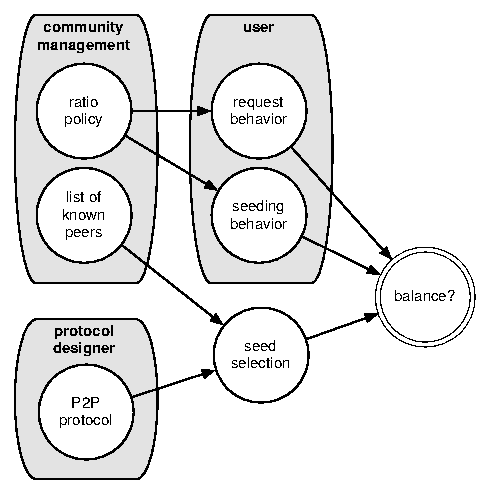
\includegraphics[width=0.7\textwidth]{pics/p2psys_balance.pdf}
	\caption{System properties and its relation to P2P balance \cite{2011:managesupplydemand:meulpolder}.}.
	\label{fig:sysbalance}
\end{figure}

% balance -> not sustain
\citeauthor{2011:managesupplydemand:meulpolder} in his work illustrated the relation between various P2P system properties and its relation to system balance. The illustration shown in figure \ref{fig:sysbalance}. Request and seeding behavior is another term of user downloading and uploading behavior, respectively. Seed selection is one part that responsible for choosing which peer to seed. In \cite{2011:managesupplydemand:meulpolder}, \citeauthor{2011:managesupplydemand:meulpolder} showed that using naive random seeding behavior is not sufficient to make P2P system balance. Unbalance system can lead to unsustainable community. Therefore, it is important to work study seeding behavior for each peer by the implementation of credit mining.

\section{Document Structure}
This thesis is structured as follows. Chapter 2 discusses problem we intend to solve and related work of it. Chapter 3 presents the design of credit mining system integrated with Tribler. Chapter 4 shows the core algorithm that we propose in credit mining system. Implementation of the mechanism and its experiment will be elaborated in chapter 5. Chapter 6 shows performance of credit mining system. At the end, chapter 7 concludes the work mentioning possible future work.


